%%
%% File: protokoll_whitelightgeneration.tex
	%% Author: Dominic Stuehler <dominic.stuehler@gmx.net>
	%% Created: Sa 30. Okt 15:53:59 CEST 2010
%% Copyright: Dominic Stuehler, 2010
%%
%% Description: Simple template in latex for protocols.
%%
%% NOTE: This document may be changed/modified and (re)distributed.
%%	 If you do so, please name always the author of the first
%%	 version of this document.
%%

\input{header}

%% Main 
\begin{document}

% Title
\titlehead{Fortgeschrittenenpraktikum WS 11/12\hfill\raisebox{-0.25cm}{\includegraphics[scale=0.06]{fau}}}
\subject{Praktikumsprotokoll}
\title{White-light generation}
\subtitle{}
\author{Dominic Stühler, Sebastian Fries}
\publishers{Gruppe 190}
\date{9.\,November 2011}
\maketitle

% Lists 
\newpage
\tableofcontents 
\listoffigures
\listoftables
\newpage

% Here goes content...
\section{Versuchsvorbereitung}
In einer photonischen Kristallfaser wird aus infrarotem, gepulstem Laserlicht ein Superkontinuum erzeugt. Dieses wird anschließend spektral untersucht. 

\subsection{Grundwissen und Grundlagen}
\subsubsection{Das Linsenteleskop}
Mit Hilfe eines Linsenteleskops werden Gegenstande betrachtet, die weit entfernt sind. Die Wirkung des Teleskops besteht darin, dass es den Sehwinkel vergrößert, so dass der Gegenstand naher erscheint. Es besteht aus zwei Sammellinsen, Objektiv und Okular, wobei das erstere ein reelles umgekehrtes Bild erzeugt, und das letztere zum Betrachten dieses Bildes dient.
Wenn der betrachtete Gegenstand sehr weit entfernt ist, ist die Bildweite gleich der Objektivbrennweite $f_{Ob}$. Da die beiden Linsen gerade $f_{Ob} + f_{Ok}$ ($f_{Ok}$ ist die Brennweite des Okulars) voneinander entfernt sind, ergibt sich die Vergrößerung zu 
$$v_T=\frac{f_{Ob}}{f_{Ok}}$$
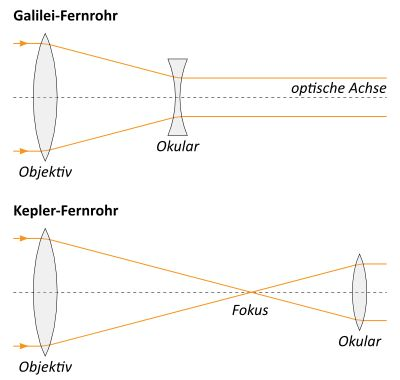
\includegraphics[scale=1]{1.jpg} 


\subsubsection{Lichtleitung in Glasfasern}
Wenn ein Lichtbündel an der Stirnfläche in eine dünne Glasfaser eintritt, wird es durch vielfache Totalreflexion gehindert, die Faser wieder zu verlassen, und tritt an der anderen Stirnfläche (nur durch Absorption geschwächt) wieder aus. Die Faser kann dabei, wenn sie dünn genug ist, praktisch beliebig gebogen sein. Interferenz zwischen den hin- und herlaufenden Bündeln ist gestattet aber Ausbreitung nur unter gewissen Winkeln zur Faserachse (Ausbreitungsmodes). In den übrigen Richtungen tritt Auslöschung ein. \\
\includegraphics[scale=0.7]{2.jpg} 

\subsubsection{Gaußstrahlen und q-Parameter}
Ein Gauß-Strahl zeichnet sich durch ein transversales Profil gemäß einer Gauß-Kurve 
(die Amplitude des elektromagnetischen Feldes nimmt mit dem Abstand zur Ausbreitungsachse exponentiell ab) und ein longitudinales Lorentz-Profil 
(er ist an einer Stelle, der Taille, fokussiert und \enquote{zerläuft} mit zunehmendem Abstand zu ihr) aus.
Gauß-Strahlen werden zur Beschreibung der Lichtemission vieler Laser herangezogen. \\
\includegraphics[scale=0.5]{3.png} 
\\
Wenn ein Gaußstrahl auf Linsen oder Spiegel fällt, ist der resultierende Strahl wieder ein Gaußstrahl. Damit lassen sich die Regeln der Matrizenoptik aus der klassischen Optik vollständig übertragen. Definiert man den Parameter $q(z) = z + iz_0$, so wirkt die ABCD-Matrix eines optischen Elementes auf ihn gemäß
$$q_1(z)= \frac{Aq_0+B}{Cq_0+D}$$

\subsubsection{Dispersion im Medium}
Unter Dispersion versteht man die Abhängigkeit einer Größe von der Frequenz, in der Optik  speziell die von der Farbe des Lichts abhängende Ausbreitungsgeschwindigkeit des Lichts in Medien. 
Der Zusammenhang zwischen der Kreisfrequenz einer Welle und dem Betrag des Wellenvektors wird Dispersionsrelation genannt.
Bei den meisten transparenten Stoffen steigt im sichtbaren Bereich der Brechungsindex mit der Frequenz an. Der positiven Ableitung $\frac{dn}{d\omega}$ entspricht $\frac{dn}{d\lambda} < 0$.

\subsubsection{Elektrisches Feld einer ebenen Welle}
Aus der Wellengleichung des elektrischen Feldes für elektromagnetische Wellen
$$\Delta \vec{E}- \epsilon \epsilon_0 \mu_0 \frac{\partial^2 \vec{E}}{\partial t^2} = 0$$
erhält man als einfachste Lösung eine ebene Welle, die sich in Richtung des Wellenvektors $\vec{k}$ ausbreitet. Ihr elektrisches Feld ist dann:
$$ \vec{E}(\vec{r},t) = \vec{E_0} \cos (\omega t- \vec{k} \vec{r} + \phi )$$

\subsubsection{Das Drude-Lorentz Modell}

Metalle sind chemisch dadurch gekennzeichnet, dass sie leicht Elektronen abgeben, d.h. durch die geringe Ionisierungsenergie ihrer Valenzelektronen. Ihre typischen physikalischen Eigenschaften - hohe elektrische und thermische Leitfähigkeit, Undurchsichtigkeit, Reflexion und Glanz - beruhen auf dieser Tatsache. 
Drude und Lorentz nahmen an, die Valenzelektronen im Kristallverband gehörten nicht mehr bestimmten Atomen an, sondern bewegten sich als Gas freier Elektronen durch das Gitter der Rumpfionen.
Unter den Leistungen des Drude-Lorentz Modells, ragt die Deutung des Ohmschen Gesetzes hervor. Die Elektronen fliegen mit thermischer Geschwindigkeit v, bis sie nach der mittleren freien Weglänge l, zeitlich also nach der freien Flugdauer $\tau = l/v$ durch einen Stoß abgelenkt werden.
Im Elektrischen Feld E wird ein Elektron mit $dv/dt = -eE/m$ entgegengesetzt zur Feldrichtung beschleunigt. Innerhalb der freien Flugdauer erhält es so eine gerichtete Zusatzgeschwindigkeit $v=-eE\tau /m$, die sich der viel größeren aber völlig ungeordneten thermischen Geschwindigkeit überlagert. Beim Stoß wird diese Zusatzgeschwindigkeit i.A. wieder verlorengehen, und das Elektron muss von vorne anfangen. Im Mittel driftet es also mit $v_d = - \frac{eE\tau}{2}$ entgegen der Feldrichtung. Seine Beweglichkeit ist dann $\mu = - \frac{e\tau}{2m}$ und die Leitfähigkeit von n Elektronen pro $m^3$
$$ \sigma = en\mu =  \frac{e^2n\tau}{2m}$$
welche nicht vom Feld abhängt (Ohmsches Gesetz).

\subsubsection{Quanteneigenschaften von Photonen}

Photonen folgen der relativistischen Energie-Impuls Relation: $E^2 = (pc)^2+ m^2c^4$
Da im Standartmodell die Ruhemasse der Photonen Null ist, vereinfacht sich die E-p Relation zu $E=pc=\hbar \omega = \hbar kc$.

Photonen sind Spin-1-Teilchen und somit Bosonen. Es können also beliebig viele Photonen denselben quantenmechanischen Zustand besetzen, was unter anderem in einem Laser realisiert wird.


\subsection{Vorbereitung}

\subsubsection{Experimentelle Grundlagen}
\begin{itemize}
\item Konfiguration des kleinsten Ablenkwinkels:
\\Der Lichtstrahl durchläuft ein Prisma bei minimalem Ablenkwinkel symmetrisch, d.h. er errechnet sich zu $\delta_{min} = 2\alpha_1 - \gamma$, wobei $\alpha_1$ der Einfallswinkel (Luft/Grenzfläche) und $\gamma$ der Winkel an der Spitze des Prismas seien. $\alpha_2$ (Grenzfläche/Prisma) ergibt sich dann zu $\gamma /2$.
Eingesetzt in das Snellius'sche Brechungsgesetz $\sin(\alpha_1) = n \sin(\alpha_2)$ folgt:
$$ n = \frac{\sin((\delta_{min}-\gamma)/2)}{\sin(\gamma /2)}$$

\item Sellmeier Gleichung:
\\ Die Sellmeier-Gleichung ist in der Optik eine empirisch ermittelte, funktionelle Beschreibung der Abhängigkeit des Brechungsindex n eines lichtdurchlässigen Mediums von der Wellenlänge $\lambda$ des sichtbaren Lichts. Sie lautet:
$$ n^2(\lambda) = A+ \frac{B_1 \lambda^2 }{ \lambda^2- C_1}+ \frac{B_2 \lambda^2 }{ \lambda^2- C_2}+ \frac{B_3 \lambda^2 }{ \lambda^2- C_3}+...$$

A, $B_i$, $C_i$ seien Materialkonstanten. Aus der Gleichung sieht man, dass die $C_i$ Quadrate von Resonanzfrequenzen sein müssen, von daher ist die Gleichung in der Nähe der Punkte $\lambda^2 =C_i$ nicht mehr sinnvoll. Physikalisch liegen hier Gebiete anomaler Dispersion vor $dn/d\lambda >0$.

\item Prismenspektrometer:
\\Für ein Prismenspektrometer braucht man im einfachsten Fall eine Lichtquelle, ggf. einen optischen Spalt (um das Licht auf das Prisma zu fokussieren), ein optisches Prisma und eine Detektorfläche. 
Der Einsatz von zwei Prismen hat den Vorteil, dass man durch die Raumgeometrie den Strahl wieder parallel zur optischen Achse ausrichten kann. Ausserdem können "unerwünschte" Nebenfrequenzen besser ausgeblendet werden, die wegen $n=n(\lambda)$ diese nicht mehr parallel zur optischen Achse verlaufen.

\item Durchmesser eines Lichtstrahls:
\\Wenn die Intensität eines Lichtstrahles einer Gauß-Verteilung folgt, also z.B. $I(r) = I_0 e^{-2r^2/w^2}$ kann man den Radius des Lichtstrahles als den Abstand von der optischen Achse definieren bei dem die Intensität auf $1/e^2$ ihres  Maximalwertes gefallen ist.
Abgesehen davon gibt es weitere Definitionen des Durchmessers, z.B. $D4\sigma$, knife-edge (siehe unten) und D86.

\item Strahltaille im Fokus einer Linse:
\\
\includegraphics[scale=0.5]{4.jpg} 
\\
Der Strahl m�ge vor dem Auftreffen auf die Linse parallel zur optischen Achse verlaufen:
$$ \Rightarrow \binom{r(z)}{\alpha(z)} = \binom{r}{0} $$
Mit den ABCD-Matrizen von Linse und Translation
$$L = \begin{pmatrix} 1 & 0 \\ -\frac{1}{f} & 1 \end{pmatrix} , T = \begin{pmatrix} 1 & d \\ 0 & 1 \end{pmatrix}$$
und $d=f$ erhält man:
$$ \binom{r(z=f)}{\alpha(z=f)}= \begin{pmatrix} 1 & d \\ 0 & 1 \end{pmatrix} \begin{pmatrix} 1 & 0 \\ -\frac{1}{f} & 1 \end{pmatrix} \binom{r}{0}= \binom{0}{-r/f}$$
$\Rightarrow r(z=f) = 0$ (Radius der Strahltaille im Fokus) 

\item Knife-Edge Methode:
\\
Es wird wie folgt vorgegangen: Man schneidet einen Teil eines Laserstrahl mit einem Messer ab und misst die Intensität des abgeschnitten Strahls als Funktion der Position des Messers. Die gemessene Kurve ist das Integral der Randverteilung des Strahls, beginnt mit maximaler Strahlleistung und fällt monoton auf Null. Der Durchmesser des Strahls ist dann definiert als der Abstand der Punkte mit 0.1/0.9 (bzw. 0.2/0.8) der Maximalleistung.

\end{itemize}
\subsubsection{Glasfasern und Photonische Kristallfasern}
\begin{itemize}
\item Die numerische Apertur:
\\Die numerische Apertur NA beschreibt das Vermögen eines optischen Elements, Licht zu fokussieren. Bei Objektiven bestimmt sie die minimale Größe des in seinem Fokus erzeugbaren Lichtflecks.
Bei einer Glasfaser berechnet sie sich zu $NA = \sqrt{{n^2}_1-{n^2}_2}$. $n_1$, $n_2$ sind die Brechungsindizes des Kerns bzw. des Mantels.
Die NA eines Mikroskopobjektivs ist definiert als $NA = n \sin{\alpha}$, wobei n der Brechungsindex des Immersionsmediums (Material zwischen Objektiv und Fokus) und $\alpha$ der halbe objektseitige Öffnungswinkel (Akzeptanzwinkel) ist.
Wenn die Werte der beiden Numerischen Aperturen nahe beieinander sind, ist eine gute Einkopplung möglich.

\item Photonische Kristallfasern:
\\ Bei der photonische Kristallfaser ist ein Gitter aus winzigen, parallelen Luftkanälen entlang der Faser eingebettet. Die regelmäßige Anordnung dieser Kanäle führt dazu, dass Licht im Kern der Faser gefangen wird. Dadurch kann ein Lichtstrahl, der sich fast vollständig im Bereich des niedrigeren Brechungsindex befindet, unter Beibehaltung des transversalen Intensitätsprofils der Grundmode kilometerweit übertragen werden. 

\end{itemize}
\subsubsection{Pulspropagation}
\begin{itemize}
\item Trägerfrequenz und instantane Frequenz:
\\
\\ Während die Trägerfrequenz eines Pulses zeitlich periodisch ist, ist es dessen instantane nicht. Technisch gesehen ist die instantane Frequenz die Zeitableitung der Oszillationsphase: 
$$ \nu(t) = \frac{1}{2\pi} \frac{d\phi}{dt}$$

\item Auswirkung der Dispersion auf einen Lichtpuls:
\\ 
\\Da ein einzelner Lichtpuls ein vergleichsweise breites Spektrum hat, breiten sich die einzelnen Frequenzen insbesondere in einer Glasfaser mit verschiedenen Geschwindigkeiten aus, da sie unterschiedliche Strecken zurücklegen müssen. Dadurch verbreitert sich der Puls und kann in ungünstigen Fällen sogar mit benachbarten Lichtpulsen überlappen.

\item Verknüpfung zwischen Zeit und Frequenzbild eines Impulses:
\\ 
\\Wenn man z.B. einen Gauß'schen Puls mit $ E(t)= E_0e^{i\omega_0 t}e^{-(2t/\tau\sqrt{ln2})^2}$ betrachtet, der die Halbwertsbreite $\tau$ besitzt, so wird sein Frequenzspektrum durch seine Fouriertransformierte berechnet. 
$$ \epsilon(\omega) = \frac{E_0}{\sqrt{2 \pi}} {\int\limits_{-T/2}}^{T/2}e^{i(\omega - \omega_0) t}e^{-(2t/\tau\sqrt{ln2})^2} dt \approx E_0 e^{-[2(\omega - \omega_0)/\Delta\omega\sqrt{ln2}]^2}$$
wenn bei sehr kurzem Pulsabstand $T/2 \rightarrow \infty$ genommen wird. Man findet wieder eine Gauß'sche Verteilung, diesmal im Frequenzbereich. Für $\Delta\omega$ und $\tau$ gilt dann: $\Delta\omega \cdot \tau = 8/ln2 $.

\end{itemize}
\subsubsection{Superkontinuumserzeugung}
\begin{itemize}
\item Berechnung der Polarisation bei zwei monochromatischen Feldern:
\\ 
\\Der Term der Polarisation zweiter Ordnung ist gegeben als
$$ P^{(2)}=\epsilon_0 \chi^{(2)}(\omega)E^2_0\cos^2(\alpha) = \frac{1}{2}\epsilon_0 \chi^{(2)}(\omega) E^2_0 [\cos(2 \alpha) + 1] $$
mit $\alpha = \omega t - \vec{k}\vec{r} +\phi$ ($\phi$ sei eine beliebige Phase). Wie man daraus ableiten kann, verdoppelt sich u.A. die Frequenz des Elektrischen Feldes.
\\
In der dritten Ordnung gilt dann:
$$ P^{(3)}=\epsilon_0 \chi^{(3)}(\omega)E^3_0\cos^3(\alpha) = \frac{1}{4}\epsilon_0 \chi^{(3)}(\omega) E^3_0 [\cos(3 \alpha) + 3\cos(\alpha)] $$
Es entstehen also zum einen Wellen mit dreifacher Frequenz aber auch Wellen mit der Ausgangsfrequenz.

\item Energie- und Impulserhaltung bei der Vier-Wellen-Mischung:
\\
\\
Bei der Vier-Wellen-Mischung lassen sich Energie- und Impulserhaltung formulieren als
$$2\omega_0 = \omega_1 + \omega_2 $$
$$2\vec{k_0} = \vec{k_1} + \vec{k_2}$$
wenn man annimmt, dass die beiden einlaufenden Wellen gleiche Energie und gleichen Impuls haben.
Aus $\hbar \omega = \hbar kc$ folgt sofort: $\vec{k_1} \Vert \vec{k_2}$, was bedeutet, dass Energie- und Impulssatz äquivalent sind.
Sei nun $\omega_1 = \omega_0 - \Delta \omega \Rightarrow \omega_2 = \omega_0 + \Delta \omega$ \\
D.h. die erhaltenen Frequenzen verteilen sich symmetrisch um die Ausgangsfrequenz.
\end{itemize}
\end{document}
%%
%% End of file `protocol_whitelightgeneration.tex`
